%======================================================================
\chapter{Software Architecture Design}
%======================================================================

% %----------------------------------------------------------------------
% \section{Stakeholder Analysis}
% %----------------------------------------------------------------------

% The successful implementation of the BorBann platform requires a understanding of all parties who may influence or be affected by the system. This stakeholder analysis identifies key individuals and groups, their interests, influence levels, and specific requirements.

%------------------------------
% \section{Domain Model}
%------------------------------

%------------------------------
% \section{Design Class Diagram}
%------------------------------

%------------------------------
\section{Sequence Diagram}
%------------------------------

\begin{figure}[htbp]
    \centering
    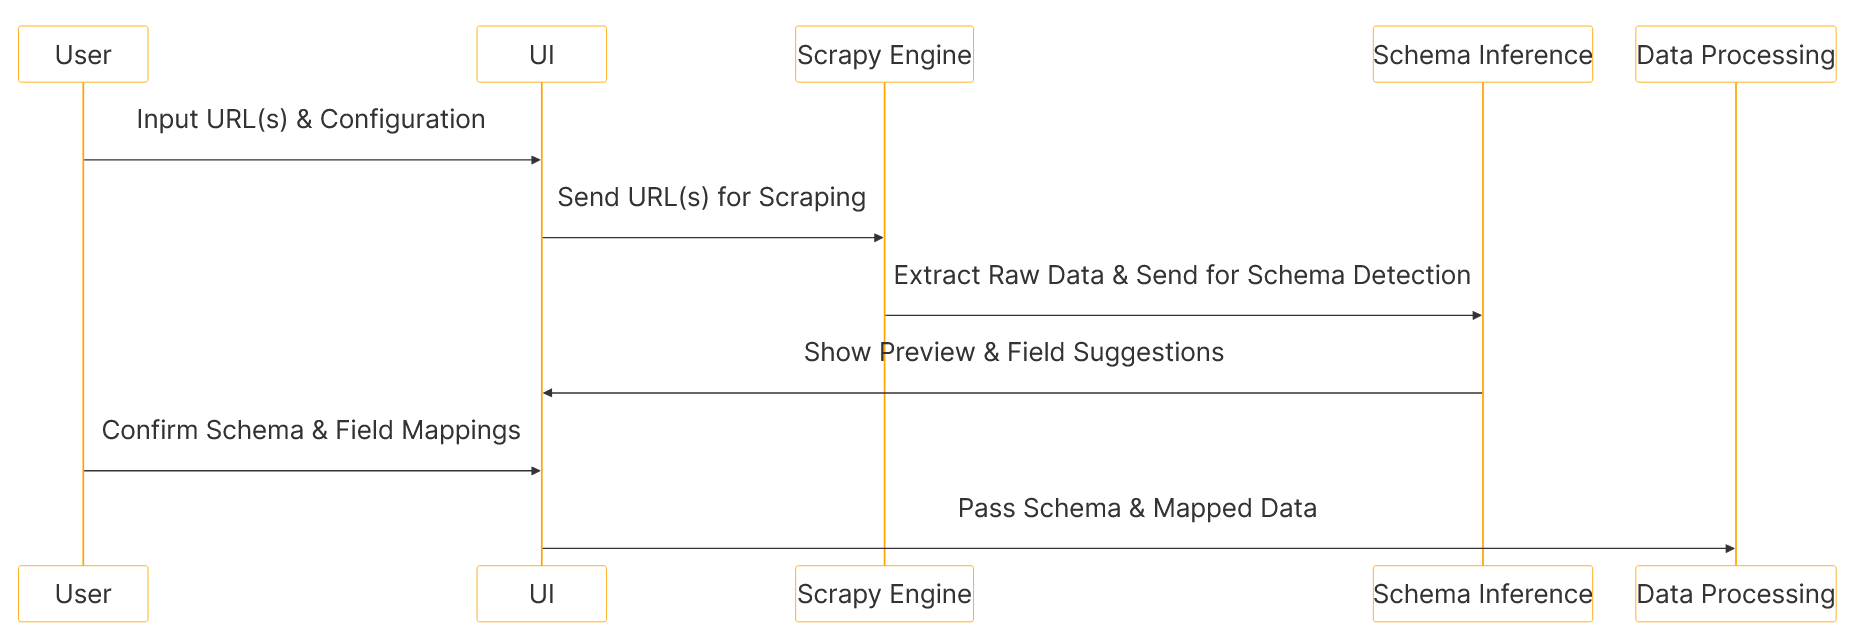
\includegraphics[width=\textwidth]{assets/sequence-diagram-pipeline.png}
    \caption{Sequence Diagram of Customizable Automated Data Integration Pipeline}
    \label{fig:sequence-diagram-data-pipeline}
\end{figure}

The sequence diagram show the flow of interactions between key components of the customizable automated data integration pipeline. The process begins with the \textbf{User}, who inputs URLs and configuration details via the \textbf{UI}. The \textbf{UI} sends the provided URLs to the \textbf{Scrapy Engine} for scraping.

Once the data is extracted, the \textbf{Scrapy Engine} forwards the raw data to the \textbf{Schema Inference} module for automatic schema detection. The \textbf{Schema Inference} module analyzes the data and returns a preview, along with field mapping suggestions, to the \textbf{UI}. The \textbf{User} then reviews the suggested schema and field mappings in the \textbf{UI}.

Upon confirmation by the \textbf{User}, the \textbf{UI} passes the finalized schema and mapped data to the \textbf{Data Processing} pipeline, where further processing and integration of the collected data occur.


% %------------------------------
% \section{Algorithm}
% %------------------------------

%------------------------------
\section{AI Component}
%------------------------------

The BorBann platform has AI components that enhance its analytical capabilities and user experience. These components work together to provide build a real estate data platform adapt to the Thai market context.
Each component integrate with each other to form a comprehensive analytics system:

\begin{itemize}
    \item The Data Integration Pipeline feeds data to the Local Contextual Analytics system
    \item Local Contextual Analytics provides features to the Explainable Price Prediction Model
    \item The Retraining Model uses data from the pipeline to create customized predictions
    \item All components share a common data model that enables smooth information flow
\end{itemize}

\subsection{Explainable Price Prediction Model}
The price prediction model delivers property price predictions with clear explanations of contributing factors.

\subsubsection{Model Architecture}

\begin{figure}[htbp]
	\centering
	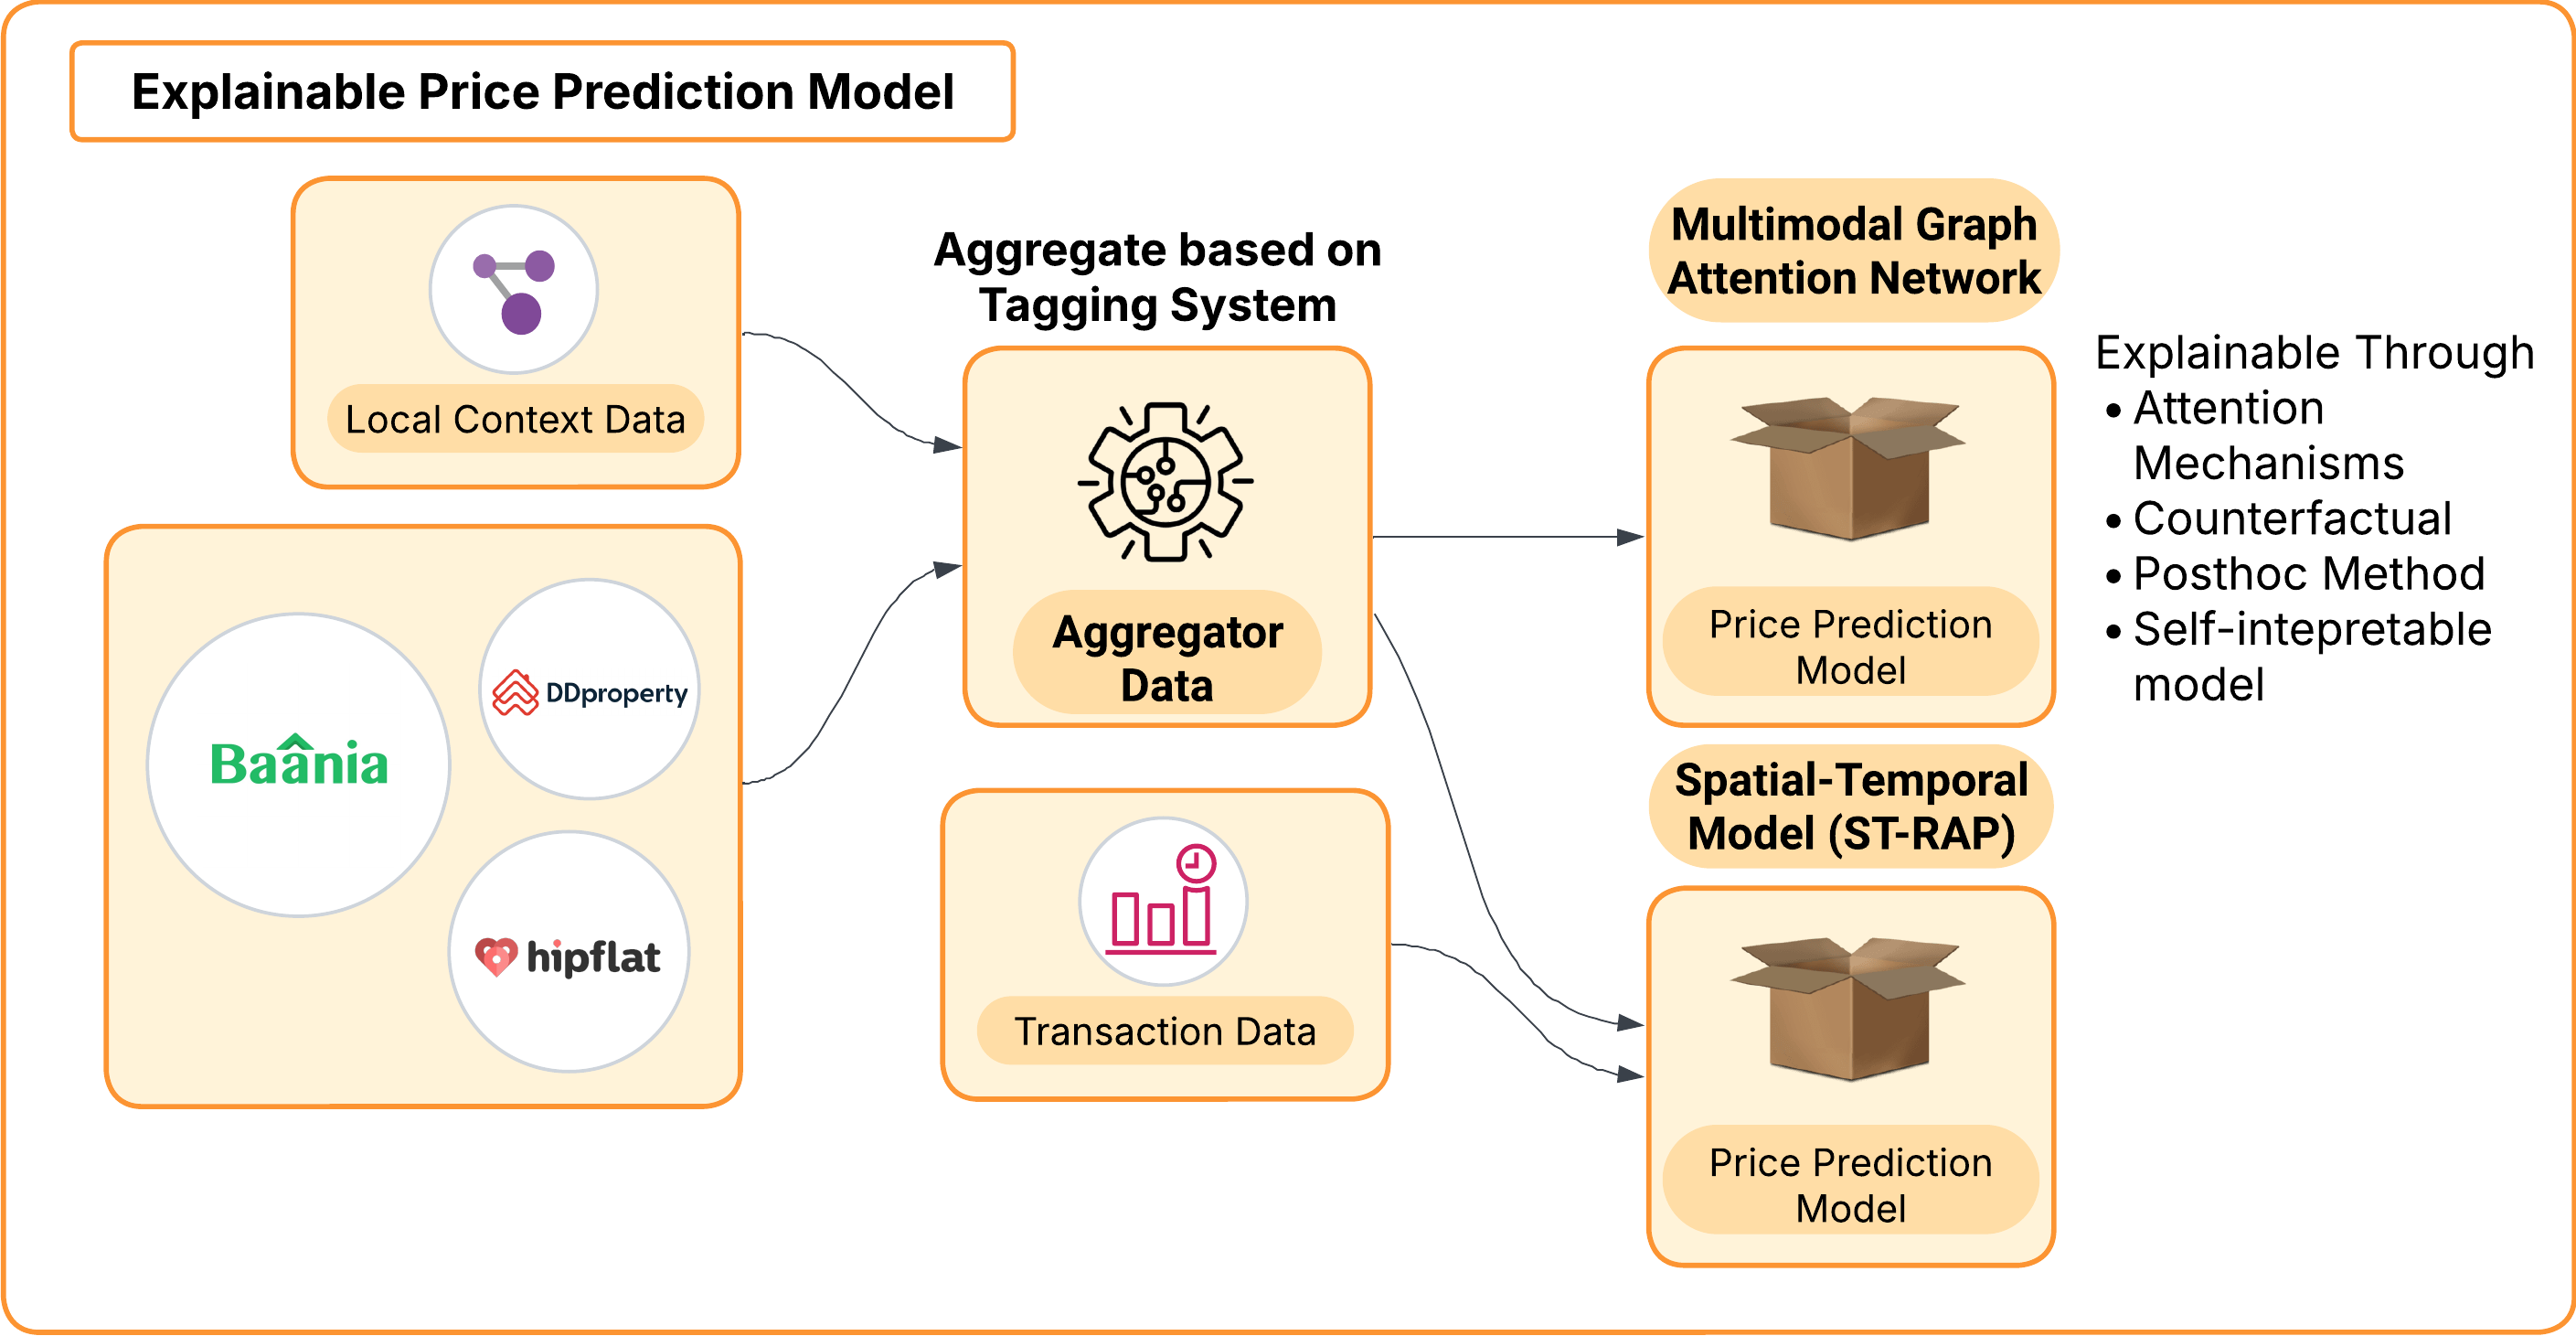
\includegraphics[width=1\textwidth]{assets/explainable-price-prediction-model.png}
	\caption{Explainable Price Prediction Data Flow}
	\label{fig:explainable-price-prediction-model-data-flow}
\end{figure}

\noindent Figure \ref{fig:explainable-price-prediction-model-data-flow} illustrates the architecture of the Explainable Price Prediction Model. The diagram shows how data flows from multiple sources (Baania, DDproperty, hipflat) and local context data into an Aggregator component that organizes information based on a tagging system. The aggregated data then feeds into two distinct prediction models: a Multimodal Graph Attention Network and a Spatial-Temporal Model (ST-RAP). The explainability features are highlighted on the right, showing how the model provides transparency through attention mechanisms, counterfactual analysis, post-hoc methods, and self-interpretable modeling approaches.

\begin{itemize}
    \item \textbf{Dual Modeling Approach:}
    \begin{itemize}
        \item \textit{Tree-based Model:} With tree-based gradient boosting models (XGBoost\cite{Chen_2016}).
        \item \textit{Multimodal Graph Attention Network:} With Multimodal Graph Attention Network\cite{veličković2018graphattentionnetworks} that is multi-modal model which can handle large graph.
        \item \textit{Spatial-Temporal Model:} Using ST-RAP\cite{ST-RAP} for facilities-property graph input and time series of real estate pricing data
    \end{itemize}
\end{itemize}

\subsubsection{Explainability Framework}
\begin{itemize}
    \item \textbf{In-model Attention:} With attention mechanism, we can look into weighted contributions of nodes, edges, or modalities
    \item \textbf{Post-hoc Explanation Module:} Uses KernelSHAP\cite{kernelshap} (Algorithm to approximate SHapley Additive exPlanations) value calculation for feature attribution.
    \item \textbf{Self-Interpretable Components:} Extracts rules from complex models and implements decision tree surrogate models that approximate complex model behavior
\end{itemize}

\subsubsection{User Interface Components}
\begin{itemize}
    \item \textbf{Interactive Visualizations:} Feature importance charts, and price trend projections with confidence intervals
    \item \textbf{Explanation Generation:} Natural language generation of price explanations and highlighting of key value drivers
\end{itemize}

\subsection{Local Contextual Analytics}
This component analyzes environmental conditions and proximity factors to evaluate property context and risk:

\subsubsection{Model Architecture}

\begin{figure}[htbp]
	\centering
	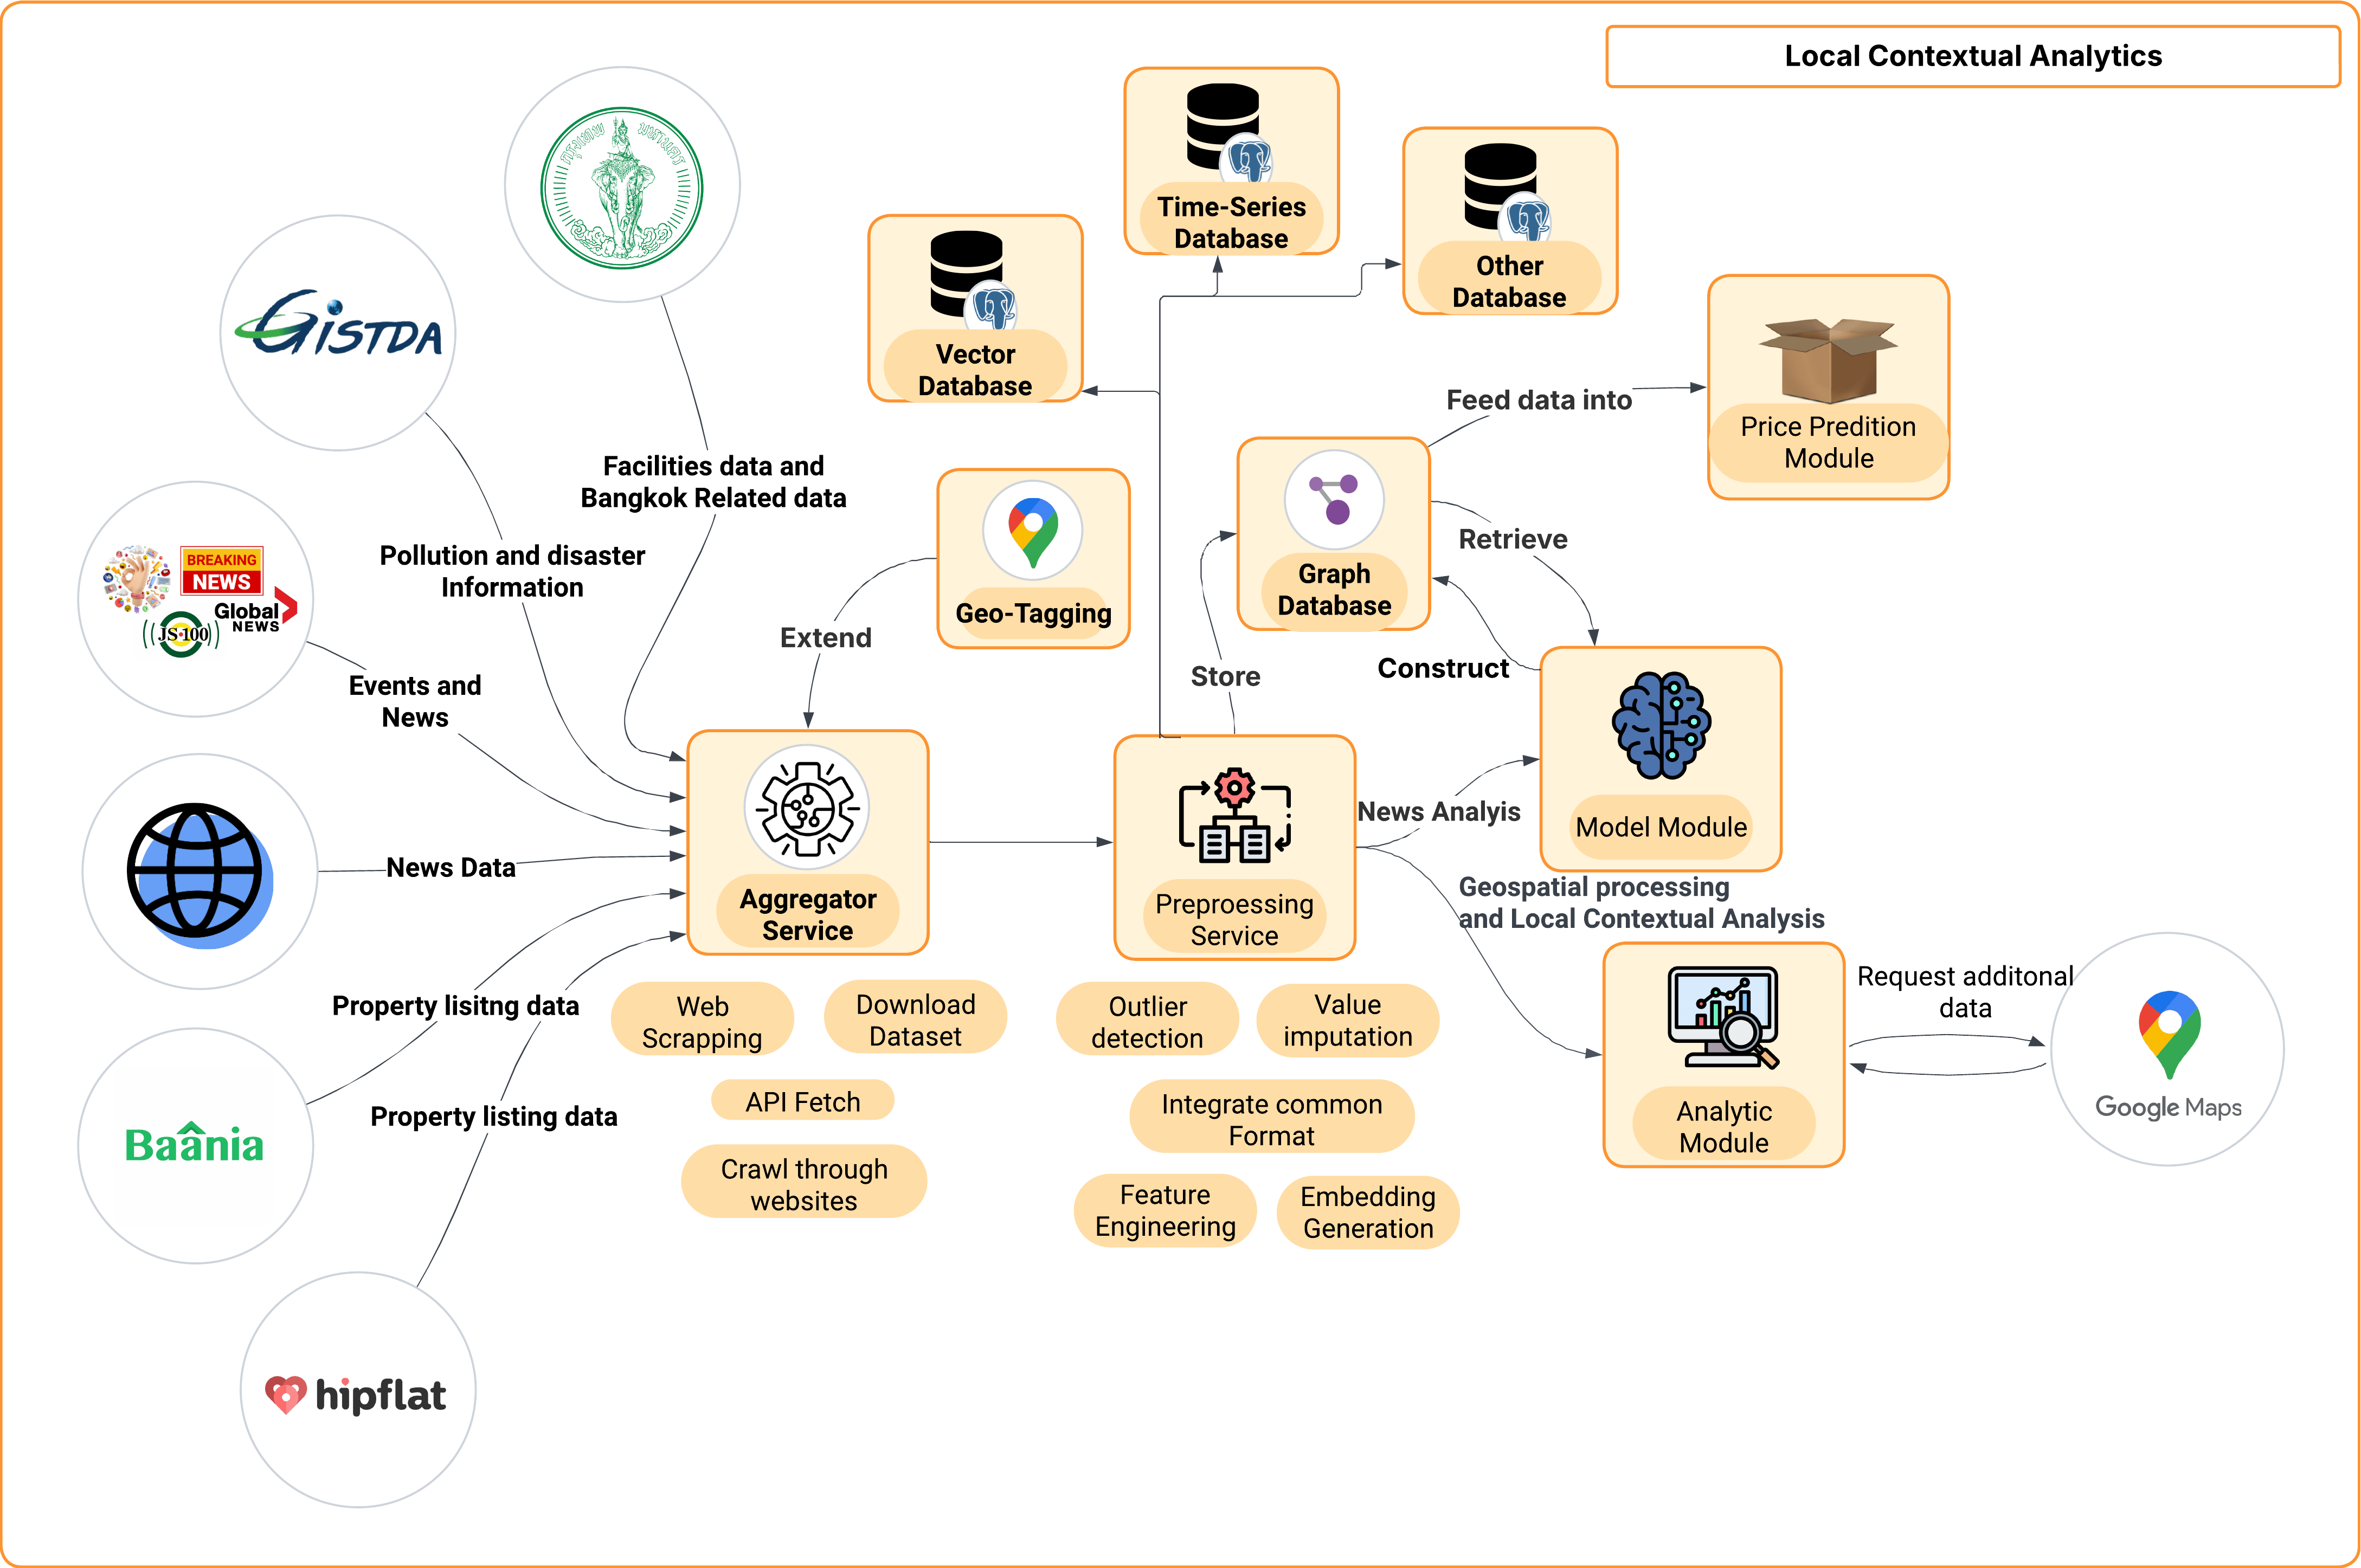
\includegraphics[width=1\textwidth]{assets/local-contextual-analytic.png}
	\caption{Local Contextual Analytic Data Flow}
	\label{fig:local-contextual-analytic-data-flow}
\end{figure}

\noindent Figure \ref{fig:local-contextual-analytic-data-flow} depicts the Local Contextual Analytics system. The diagram shows various data sources including GISTDA, Bangkok Metropolitan Administration,  news outlets, and property listing platforms (Baania, hipflat) feeding into an Aggregator Service. This service collects different types of data through web scraping, API fetching, and dataset downloads. The collected data undergoes preprocessing with outlier detection, value imputation, and feature engineering before being stored in specialized databases (Vector, Time-Series, Graph). The Model Module and Analytic Module process this information to provide geospatial analysis and local contextual insights that ultimately feed into the Price Prediction Module.

\begin{itemize}
    \item \textbf{Graph Database:} Stores heterogeneous data in Neo4J or other knowledge graph database
    \item \textbf{Vector Database:} Stores embedding from preprocessing unit within PostGreSQL with pgvector that will provide vector database capabilities
    \item \textbf{Timeseries Database:} Stores time-series data withtin Timescale
    \item \textbf{Relational Database:} Stores relational data in PostgreSQL
    \item \textbf{NoSQL Database:} Stores unstructured data within MongoDB
    \item \textbf{Model Module:} 
    \begin{itemize}
        \item Heterogeneous Graph Construction using k-NN or GCN
        \item GCN models for spatial relationships
        \item NLP models for news analysis
    \end{itemize}
    \item \textbf{Price Prediction Module:} Integrated model consuming all processed features
\end{itemize}

\subsubsection{Analytics Capabilities}
\begin{itemize}
    \item \textbf{Climate and Environmental Analysis:} Evaluates climate risk, pollution levels, and disaster assessment
    \item \textbf{Proximity Analysis:} Evaluates nearby locations and facilities, analyzing relationships between facilities
    \item \textbf{News Integration:} Incorporates local news into property assessment
\end{itemize}

\subsection{Customizable Automated Data Integration Pipeline}
This pipeline enables non-technical users to connect any data source into a unified system:

\subsubsection{LLM Module}

\begin{figure}[htbp]
	\centering
	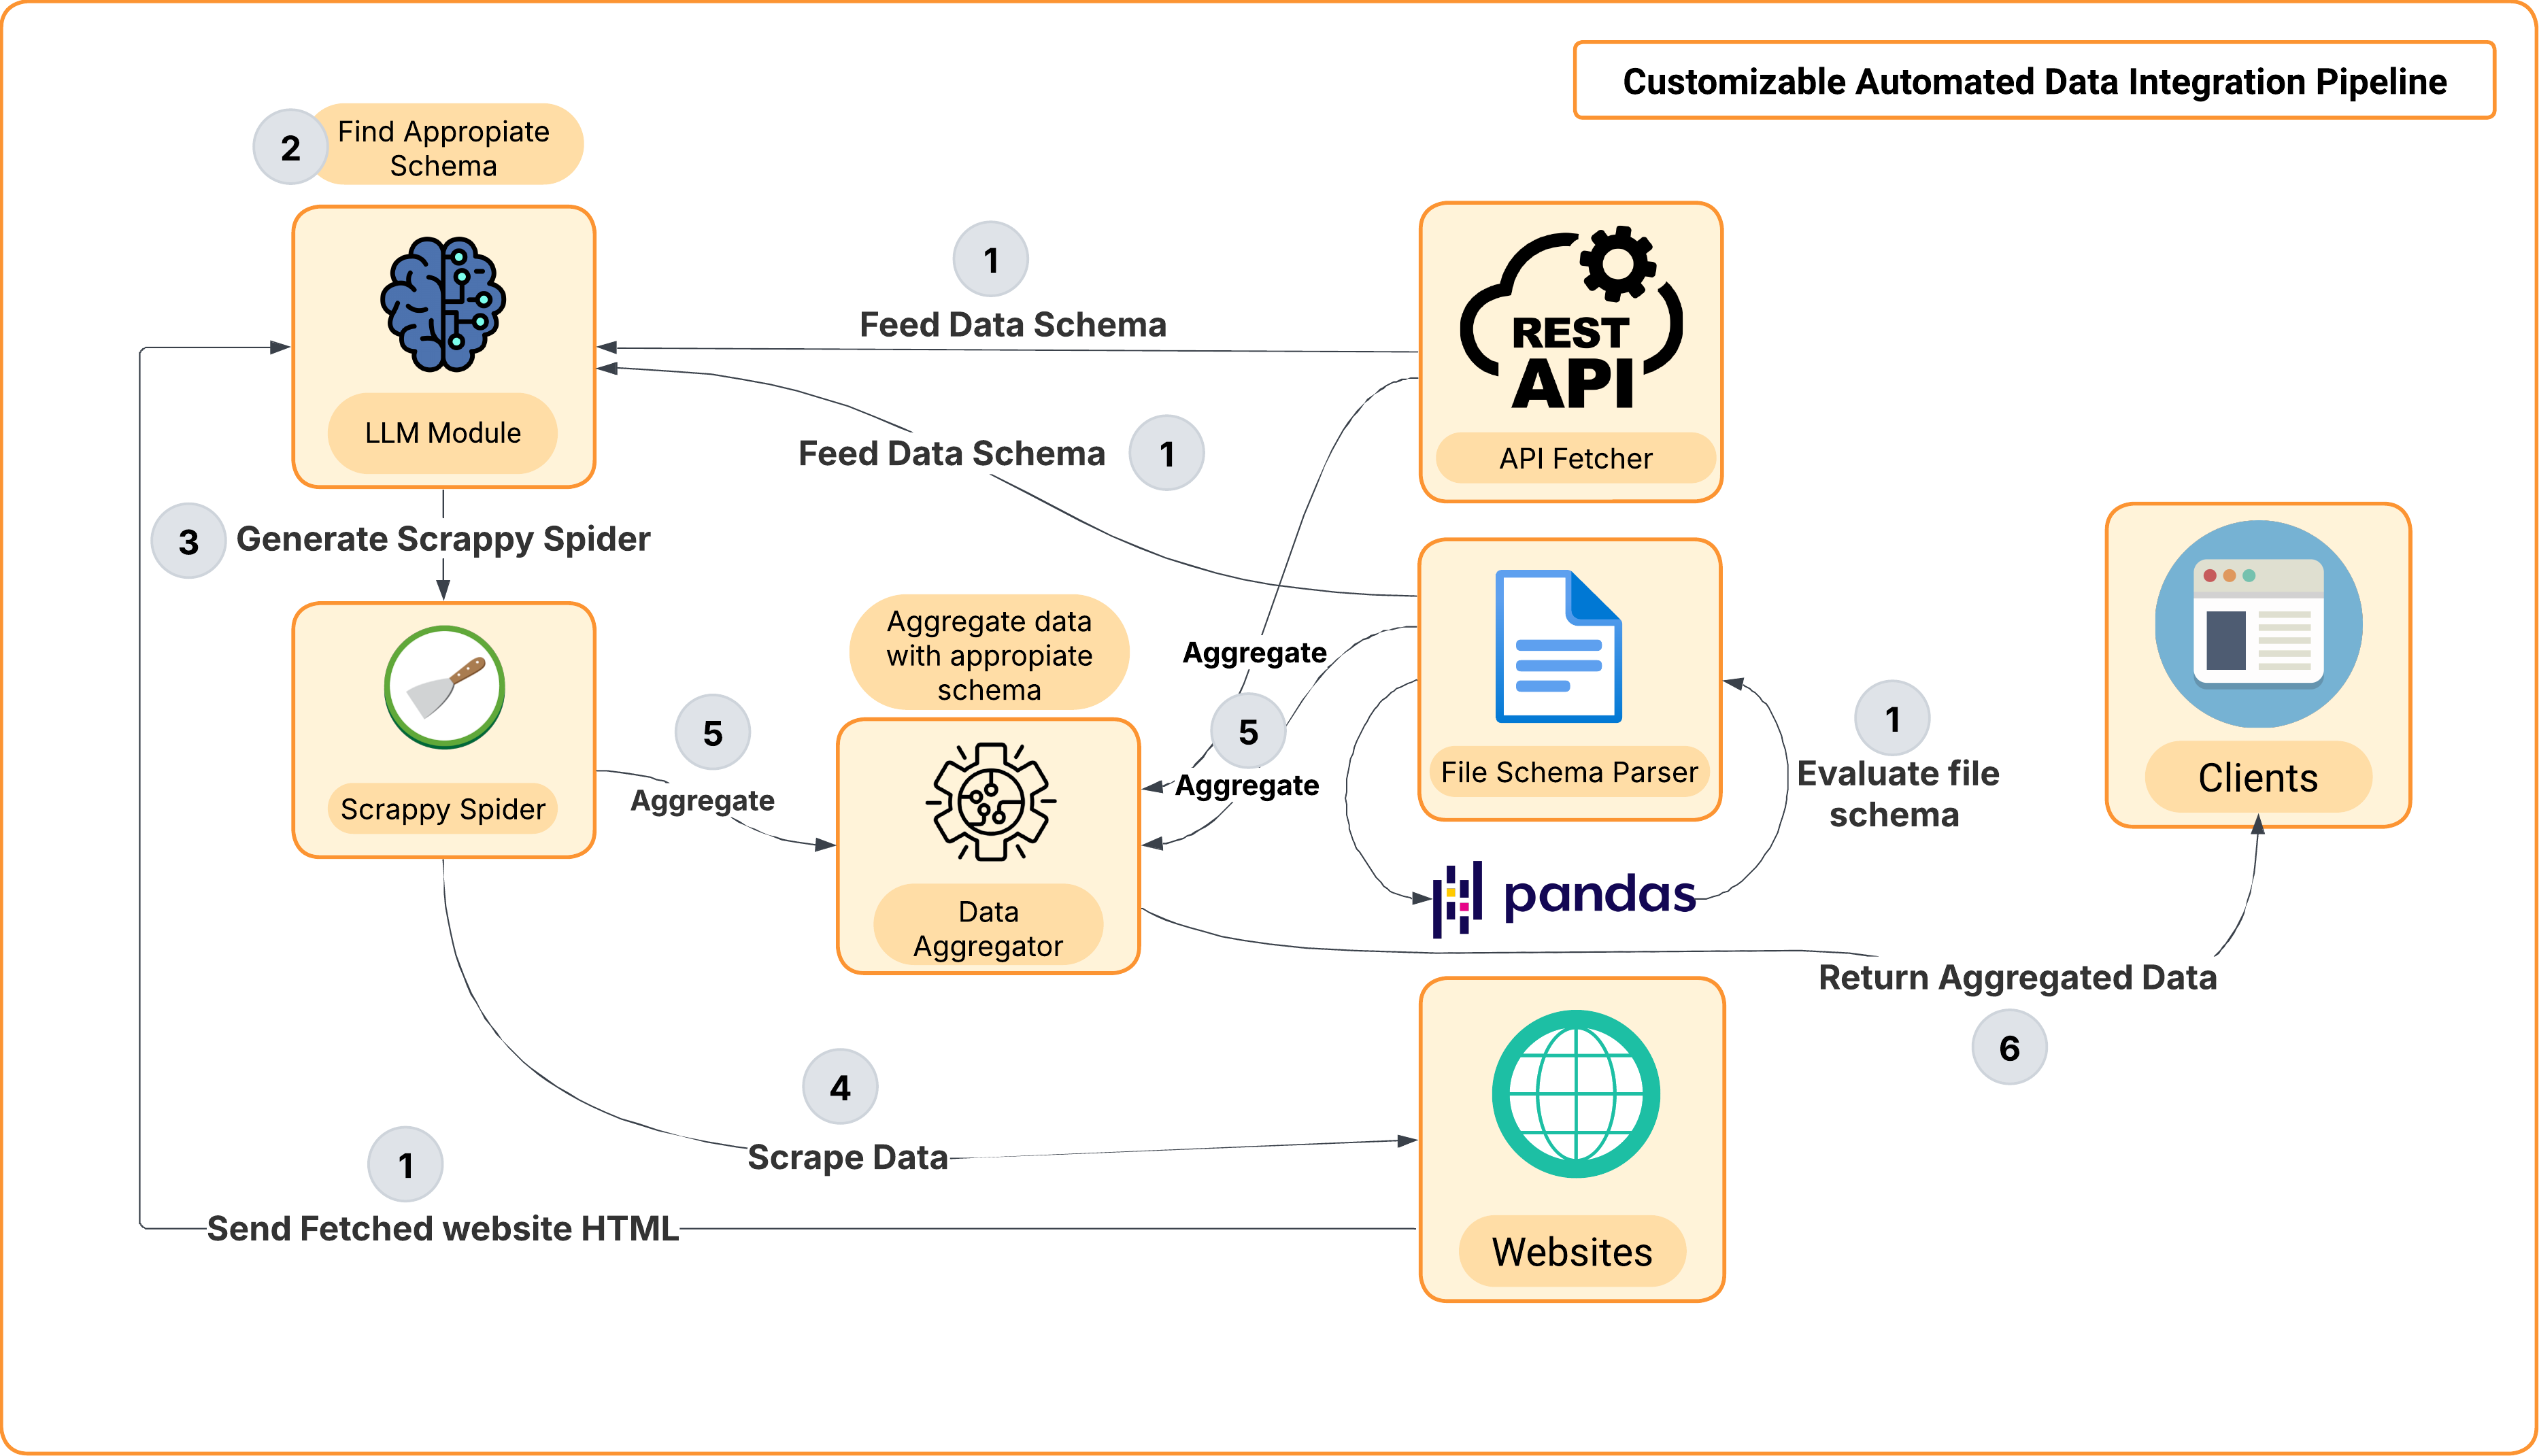
\includegraphics[width=1\textwidth]{assets/customizable-automated-data-integration-pipeline.png}
	\caption{Customizable Automated Data Pipeline Data Flow}
	\label{fig:customizable-automated-data-integration-pipeline-data-flow}
\end{figure}

\noindent Figure \ref{fig:customizable-automated-data-integration-pipeline-data-flow} presents the Customizable Automated Data Integration Pipeline. The workflow begins with data sources (API Fetcher, File Schema Parser, Websites) being evaluated. An LLM Module analyzes these sources to find appropriate schemas (step 2), then generates Scrappy spiders for web scraping (step 3). The spiders extract data from websites (step 4), while the Data Aggregator combines information from all sources (step 5). Finally, the aggregated data is returned to clients (step 6). This pipeline enables non-technical users to integrate diverse data sources through an automated, LLM process.

\begin{itemize}
    \item Analyzes data sources to find appropriate schemas
    \item For websites, generates Scrappy spider configurations automatically
    \item Bridges the gap between unstructured and structured data
\end{itemize}

\subsubsection{Data Processing}
\begin{itemize}
    \item \textbf{Scrappy Spider:} Dynamically generated web scrapers based on LLM analysis that extract targeted data from websites according to the determined schema
    \item \textbf{Data Aggregator:} Central component that combines data from all sources, harmonizes different schemas into a unified structure, and uses appropriate schema mapping determined by the LLM
\end{itemize}

\subsection{Retraining Model with Pipeline Data}
This component allows users to create custom prediction models by combining their pipeline data with platform data:

\subsubsection{Technical Implementation}

\begin{figure}[htbp]
	\centering
	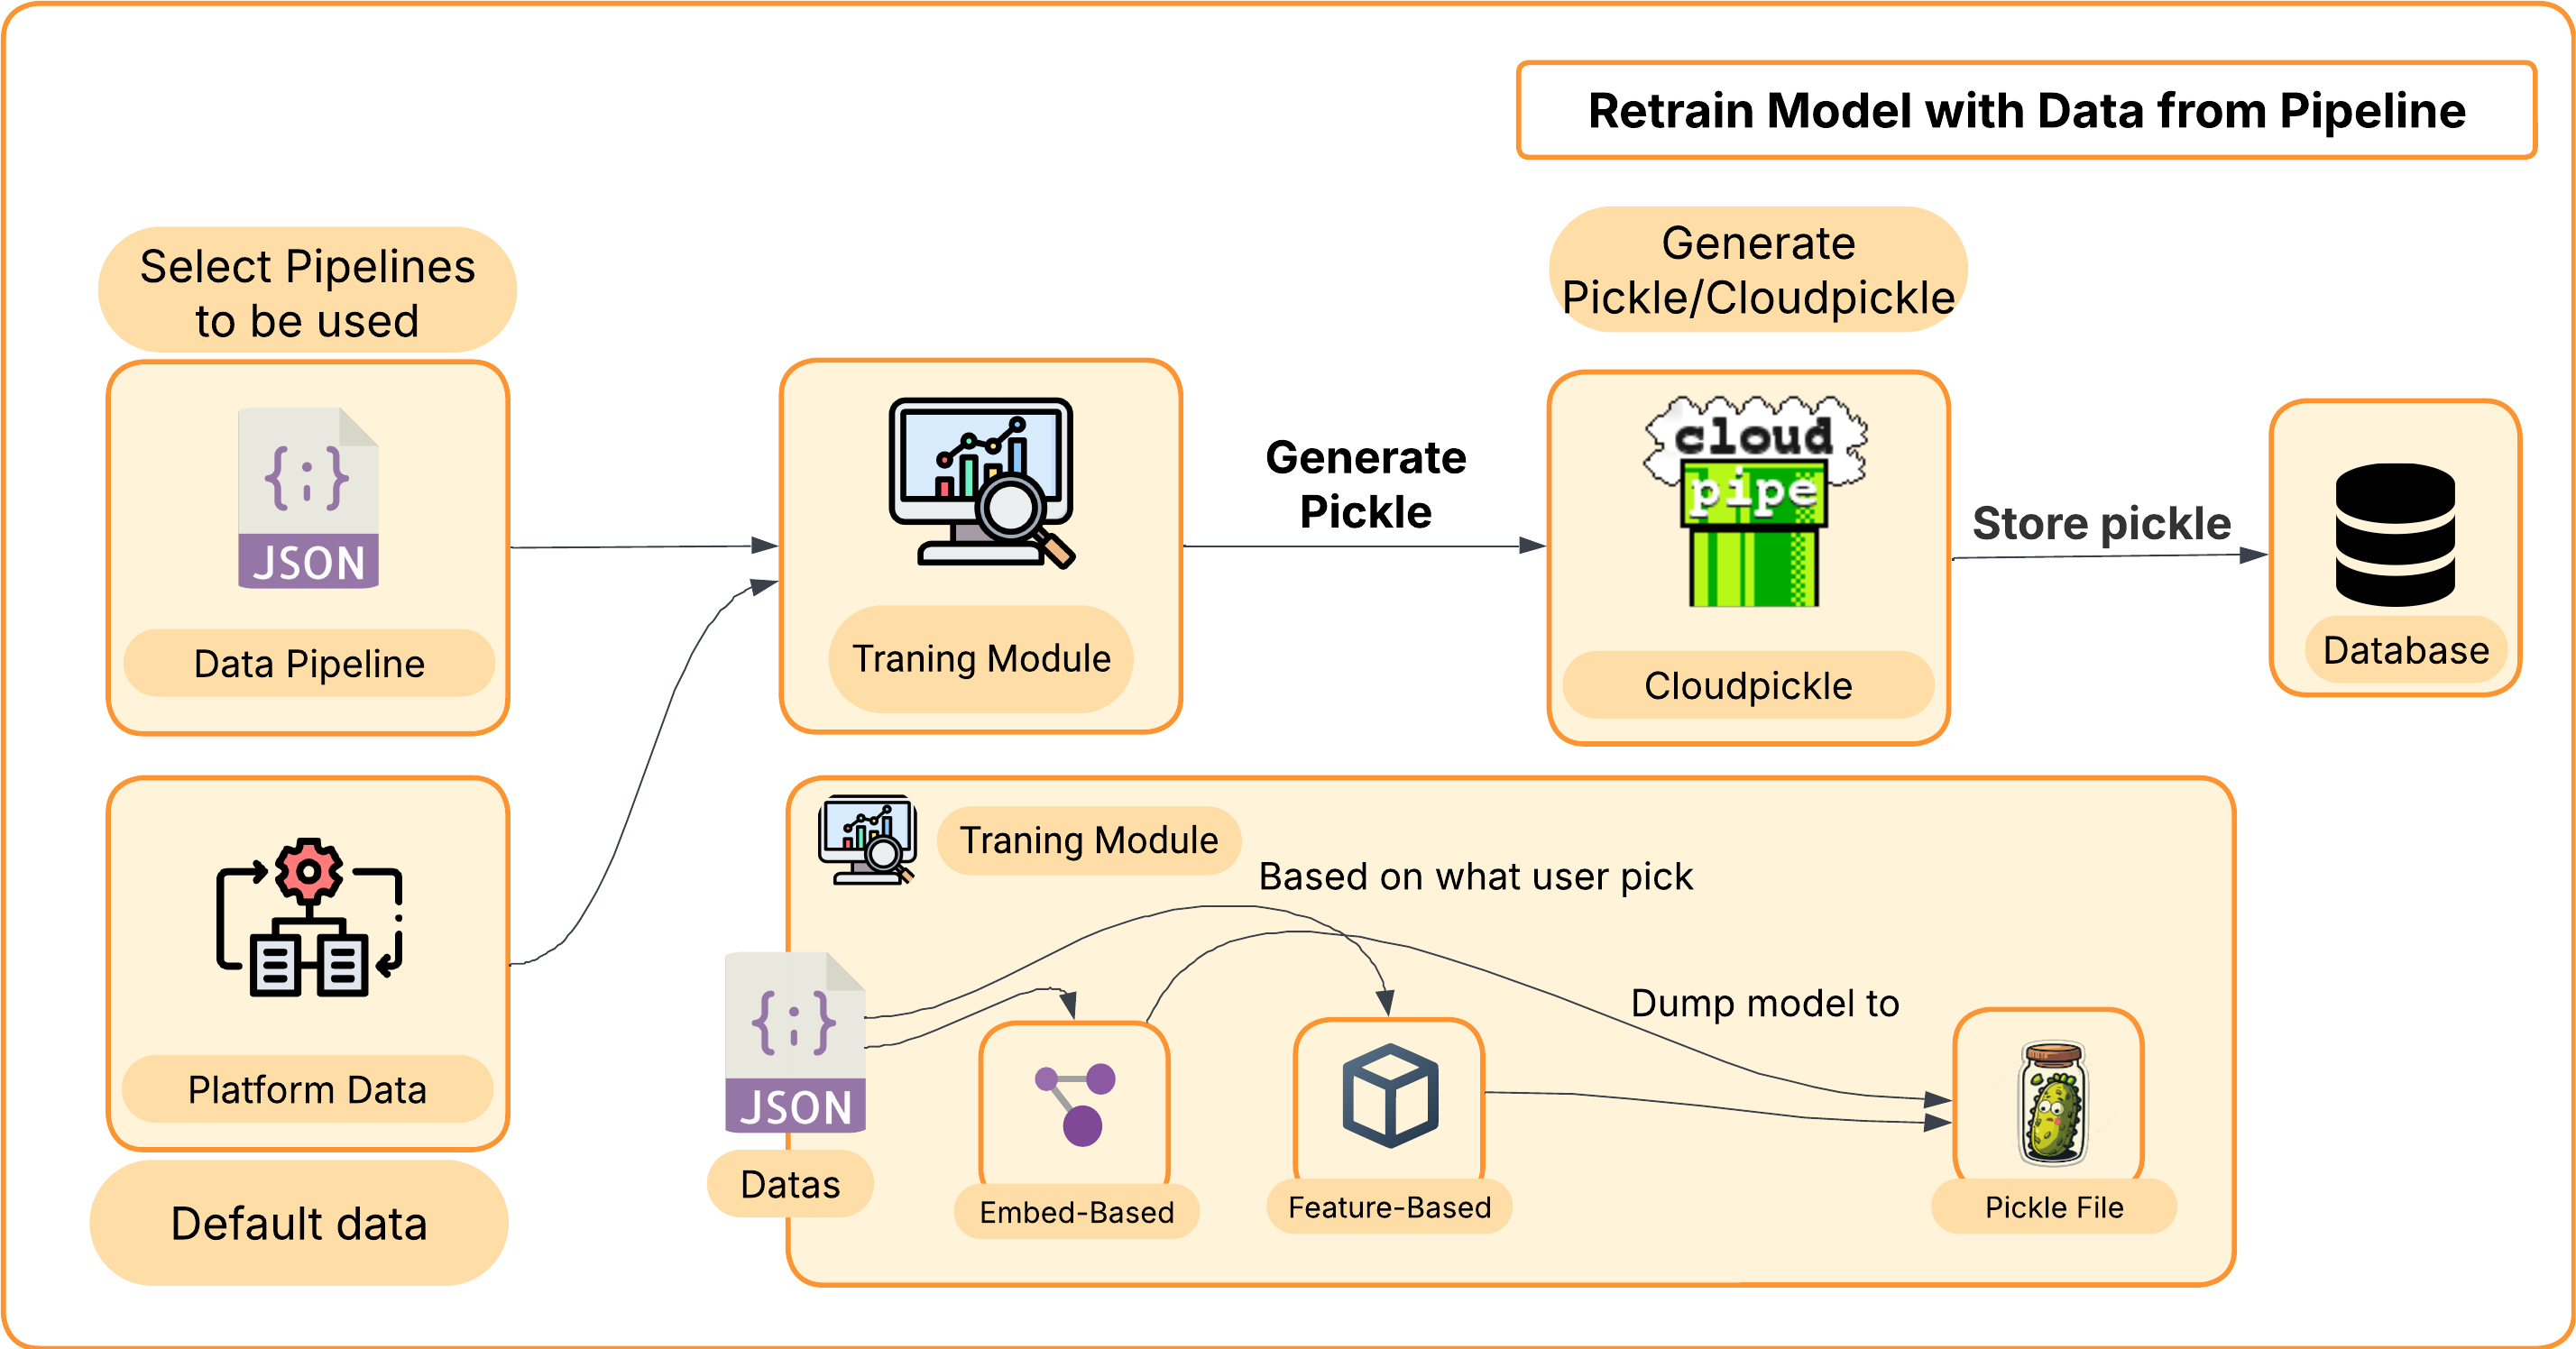
\includegraphics[width=1\textwidth]{assets/retrain-model-with-data-from-pipeline.png}
	\caption{Retrain Model with Data from Pipeline Data Flow}
	\label{fig:retrain-model-with-data-from-pipeline-data-flow}
\end{figure}

\noindent Figure \ref{fig:retrain-model-with-data-from-pipeline-data-flow} shows the Model Retraining Pipeline. The diagram illustrates how users can select pipelines and combine them with platform data to train custom models. The Training Module processes this data and allows users to choose between embed-based or feature-based modeling approaches. The system generates pickle/cloudpickle files of the trained models, which are then stored in a database for future use. This component empowers users to create specialized prediction models tailored to their specific data and requirements.

\begin{itemize}
    \item \textbf{Training Engine:} Implements automated training engine that rely on embedding-based models to avoid problem with unmatch input feature and tree-based models (for structured data), and builds parameter tuning system using random search if user doesn't specify ones.
    \item \textbf{Model Serialization:} Creates versioned model files for persistence and stores serialized models in pickle format in database with metadata
    \item \textbf{Deployment Framework:} Provides APIs for model inference, enables batch prediction, and implements monitoring for model drift detection
\end{itemize}

% \subsection{Integration Architecture}
% Each component integrate with each other to form a comprehensive analytics system:
% \begin{itemize}
%     \item The Data Integration Pipeline feeds data to the Local Contextual Analytics system
%     \item Local Contextual Analytics provides features to the Explainable Price Prediction Model
%     \item The Retraining Model uses data from the pipeline to create customized predictions
%     \item All components share a common data model that enables smooth information flow
% \end{itemize}